%!TEX root=../book.tex

\chapter{Simple Linear Regression}

\section{Overview of Simple Linear Regression}

\subsection{Uses of Simple Linear Regression}
In the last chapter we touched briefly on the idea of using the value of one variable to predict the value of another. Where correlation is used to describe the magnitude of the relationship between two variables, a tool called \textbf{simple linear regression} takes that relationship and uses it to predict the values of Variable B, given some arbitrary value of Variable A. In this context, however, we refer to the \(x\) variable as our \textbf{explanatory variable} or our \textbf{regressor} and to the \(y\) variable as the \textbf{response variable}.

So, knowing that we use regression as a predictive tool, what \textit{is} it, exactly? Well, thankfully, it's a pretty straightforward thing that we can define as:

\begin{equation}
\hat{y} = \beta_0 + \beta_1\cdot x
\label{eqn:regression01}
\end{equation}

So before we explain this equation, we need you to reach way back into those murky memories of your eighth grade math class when you were talking about the equation of a line. Remember that whole ``slope-intercept form'' lecture? Well, in case you don't, the equation of a line looks something like:
\begin{equation*}
y=m\cdot x+b
\end{equation*}
where $m$ is the slope and $b$ is the intercept. Sound familiar?

Alright, now let's compare those two equations. Aside from using different variable names, they're identical to one another. All regression boils down to is drawing lines to connect a bunch of points on the page. And here you thought it was going to be scary!

Although regression is actually a bit more than drawing a line to connect the dots, the basic idea behind it is that for two variables there exists an equation with two basic constants---a slope and an intercept---that allows us to predict the value of $Y$ if we already know $X$.

But, although we know that equation exists, how do we figure it out? To do that we'll turn to something called \textbf{least squares estimators}.

\subsection{Least Squares Fitting}

If you think back to Equation \ref{eqn:regression01}, our two coefficients were $\beta_0$ and $\beta_1$. Those refer to the population coefficients: that is, if we were able to measure every single instance of $X$ and $Y$ in all of the universe, those would be the coefficients that we could derive from the population. In most cases, however, that isn't possible and so we use least squares estimates of $\beta_0$ and $\beta_1$ which we refer to as $\hat{\beta}_0$ and $\hat{\beta}_0$ (pronounced ``beta-null hat'' and ``beta-one hat'').

We can visualize this process in Figure \ref{fig:regression01}. Here, we see a number of data points as white circles. There is also a solid black line that represents a possible line of best fit. However, are the predicted data points (solid black circles) as close to the observed data as possible? Looking at the red dashed line between our predictions and observations, it looks like we could do a better job reducing that difference.

\begin{figure}[htp]
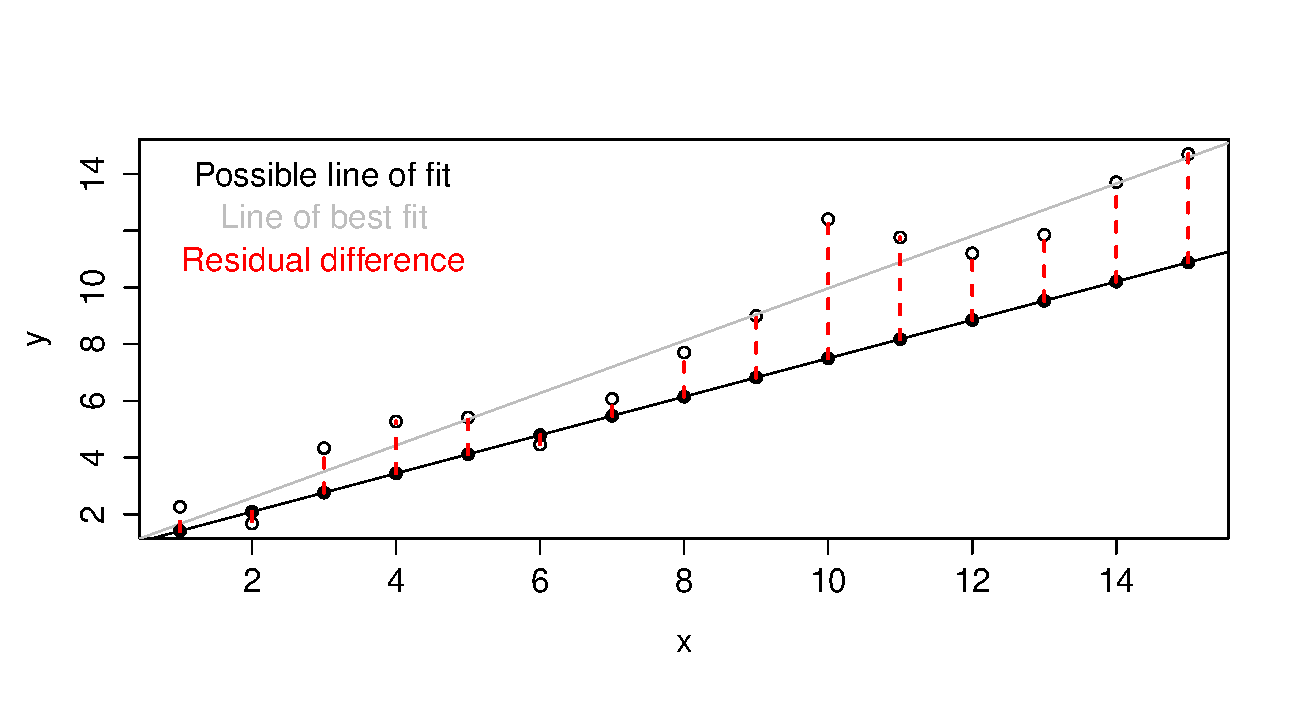
\includegraphics[width=35pc]{regression01}
\caption{Data with a least-squares line of best fit (grey), one potential line of best fit (black), and the residual difference between the predicted and observed values (red). Lease squares fitting seeks to minimize the overall distance between every observed value and predicted value, resulting in a single line of best fit.}
\label{fig:regression01}
\end{figure}

Minimizing that difference between our predicted and observed values is exactly what least squares estimation seeks to do. In fact, we can see the least squares line of best fit as the light grey line in Figure \ref{fig:regression01}. The residual difference in this line is mathematically as small as it possibly can be.

How we actually do this involves a bit of calculus so we aren't going to go into too much detail here. However, from that calculus we can derive these two estimates of our coefficients:
\begin{eqnarray*}
\hat{\beta}_1 &=& \frac{\sum_{i=1}^n\left(X_i-\bar{X}\right)\left(Y_i-\bar{Y}\right)}{\sum_{i=1}^n\left(X_i-\bar{X}\right)^2}\\
\hat{\beta}_0 &=& \bar{Y}-\hat{\beta}_1\cdot \bar{X}
\end{eqnarray*}

Thankfully, these aren't equations that you're liable to ever have to understand or use (unless you just really want to): least squares fitting is automated by every modern statistical package. Even your TI-84 calculator is happy to do it for you. The point, rather, is that given a set of data, there are these mathematical tools that we can use to attempt to model the relationship between our variables, even though this is mostly a behind-the-scenes operation.

\subsection{Coefficient of Determination}

The whole of a simple linear regression boils down to just a couple numbers, one of which is the \textbf{coefficient of determination}, denoted $R^2$ (pronounced ``R-squared''). This statistic represents the proportion of the variance seen in the data that is explained by the model.

If you think back to the chapter \textit{Measuring Uncertainty}, variance is the squared average distance of a data point from the mean. Let's take Figure \ref{fig:regression03} as an example. Here, we see that there is a regression equation fitted to the data with an $R^2=0.39$, indicating that about 39\% of the variance observed within the data is explained by the model.

\begin{figure}[htp]
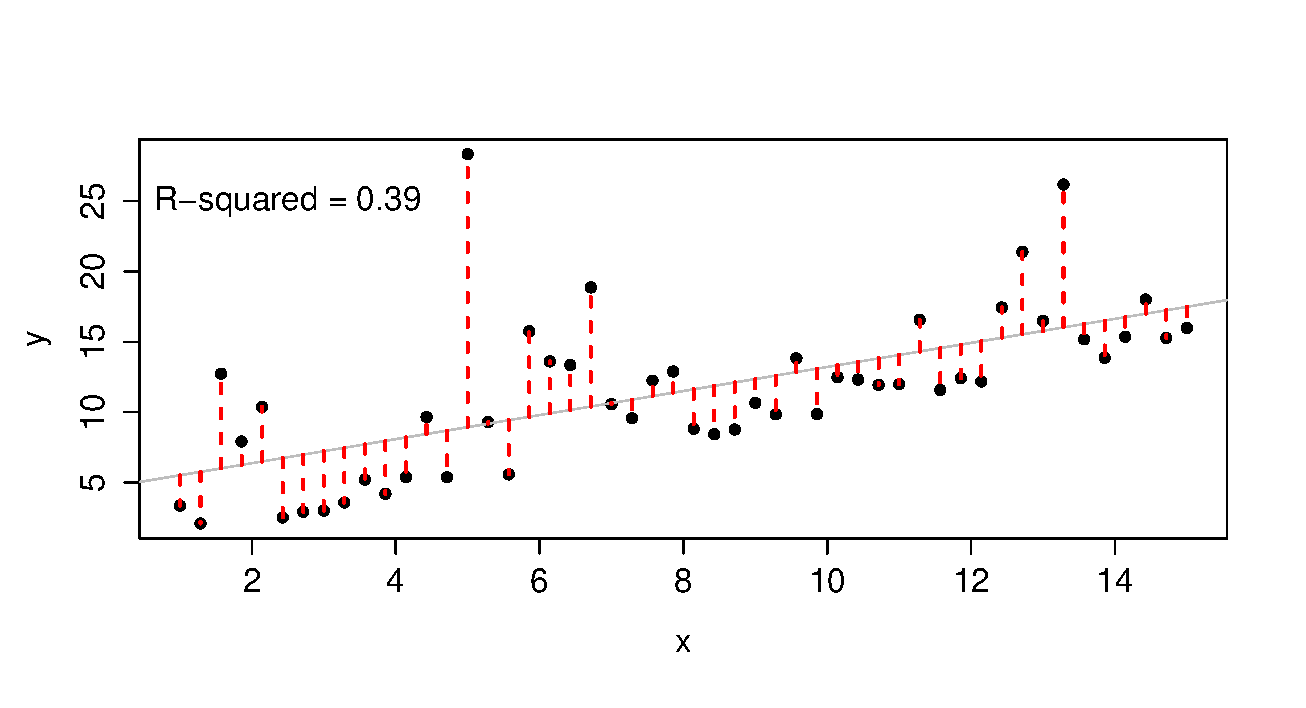
\includegraphics[width=35pc]{regression03}
\caption{Regression model with approximately 39\% of the observed variance explained.}
\label{fig:regression03}
\end{figure}

Now, it's important to recognize that the line of best fit that we've plotted doesn't describe our data perfectly. This is because there is an inherent bit of error---random variability---in any dataset (and thereby any equation that we use to model it). Given this, a better definition of Equation \ref{eqn:regression01} is:
\begin{equation}
\hat{y} = \beta_0 + \beta_1\cdot x+\epsilon
\label{eqn:regression02}
\end{equation}
where $\epsilon$ represents that error. In our example, we can see that each point does not vary above or below the regression line by an equivalent amount: if there were no error, then the distance of all of the points from the regression line, above and below, should sum out to 0. (That is, points above the line are equally far from it as are points below the line.)

The equation that we use to model our data will never be able to perfectly explain all of that random variation which is why we use the $R^2$ statistic to quantify the proportion of it that \textbf{can be} explained. Correspondingly, a larger value of $R^2$ corresponds to a model that better fits the data.

As with Pearson's $r$ in correlational designs, $R^2$ varies from 0 to 1. (Note: Pearson's $r$ can fall on the interval (-1, 1); however, because the coefficient of determination is squared, it can only fall on the interval (0, 1). Any negative number multiplied by another negative number will always equal a positive number.)

\subsection{Residuals}

The formal calculation of the proportion of the variance that is explained by the model is a bit more complicated than what we presented above. To understand how $R^2$ is calculated, we first need to understand the concept of \textbf{residuals}. A residual is defined as the difference between an observed and predicted value. If we look back to Figure \ref{fig:regression03}, the residuals are represented by the dashed red lines. Alternately, we can see a little more explicitly what a residual is by looking at Figure \ref{fig:regression05}. This is equivalent to the error term ($\epsilon$) that we mentioned in the previous section.

\begin{figure}[htp]
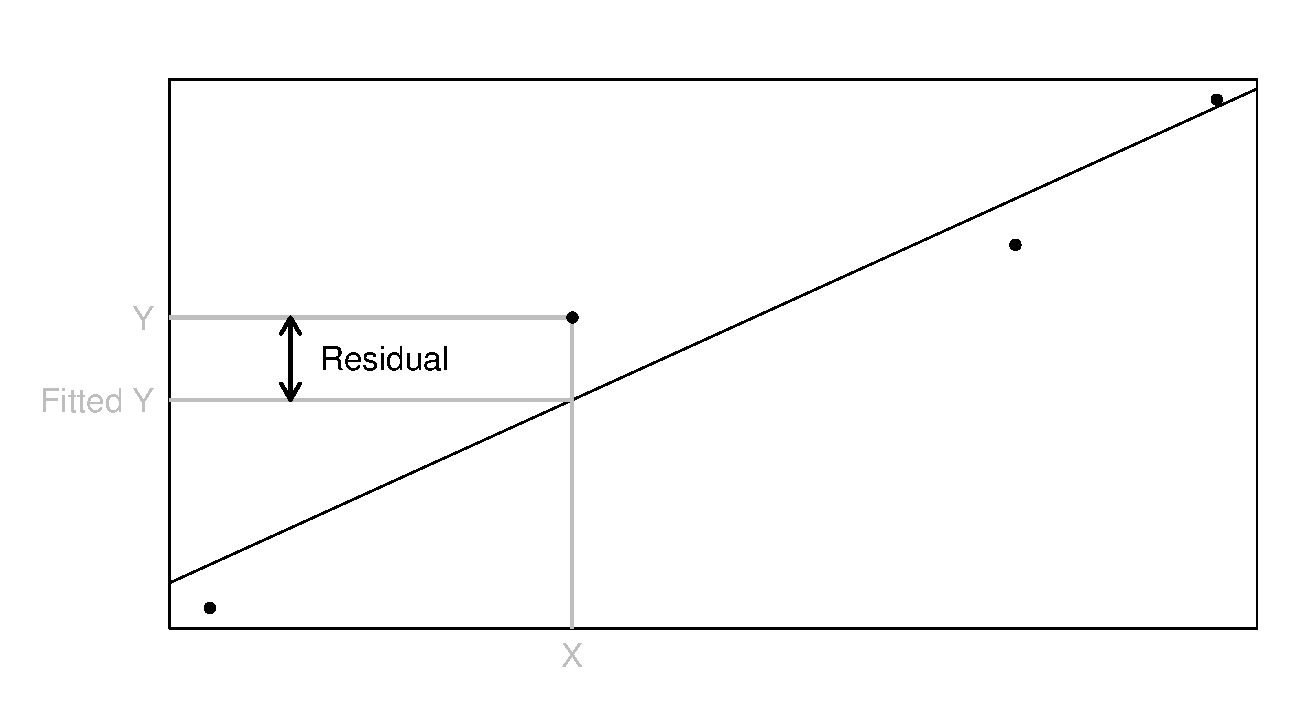
\includegraphics[width=35pc]{regression05}
\caption{A residual is the difference between an observed data point and its predicted value at a given point $X$. This represents the error that the model is unable to explain.}
\label{fig:regression05}
\end{figure}

\subsubsection{$R^2$ and Residuals}
When calculating $R^2$, we use the formula:
\begin{equation}
R^2 \equiv 1-\frac{SS_{residual}}{SS_{total}}
\end{equation}
where $SS_{residual}$ is the residual sum of squares and $SS_{total}$ is the total sum of squares. To get an idea of what these two terms mean, let's look at Figure \ref{fig:regression04}. On the left we see a representation of the total sum of squares for four data points. This is derived by finding the squared distance between each observed data point and the arithmetic mean of $y$ and adding them all together. Mathematically, we represent this as:
\begin{equation*}
SS_{total} =\sum_i \left(y_i-\bar{y}\right)^2
\end{equation*}
The idea here is that we want to find out the total distance of our data from their mean: a larger value means that the data are farther dispersed from their mean; a smaller value indicates that they all cluster closer to their mean value. (Likewise, a value closer to 0 indicates a weaker relationship between the two variables: it shows that $y$ is unaffected by the value of $x$.)

Next we have the residual sum of squares. This value represents the sum of the squared distances of each point from its predicted value. In other words, it's a measure of how accurately the data can be fitted to a line. Mathematically, we represent this as:
\begin{equation*}
SS_\text{residual}=\sum_i \left(y_i - \hat{y}_i\right)^2
\end{equation*}
As with our total sum of squares, a higher value for our residual sum of squares indicates a larger discrepancy between our predicted and observed values of $y$ whereas a smaller value indicates a better fit of the model to the data. By then comparing the ration of these two values, we can assess what proportion of the total variance our model is able to explain, and thus how good of a fit it provides.

It may help if we visualize these, as in Figure \ref{fig:regression04}. Here, the total sum of squares is represented in red on the left.  We see that the horizontal line represents the average $y$ value across our four data points---just below $2.0$. To compute the total sum of squares, we measure how far apart the $y$ value for each of our four data points is from that average and we square it. This is represented by each of the red boxes. To obtain our sum of squares, we just go ahead and add the areas of the four boxes.

You can also think of the total sum of squares as a measure of the relationship between our explanatory and response variables: if there were no relationship between them, then every single data point would be exactly on the line and our sum of squares would be $0$.

\begin{figure}[htp]
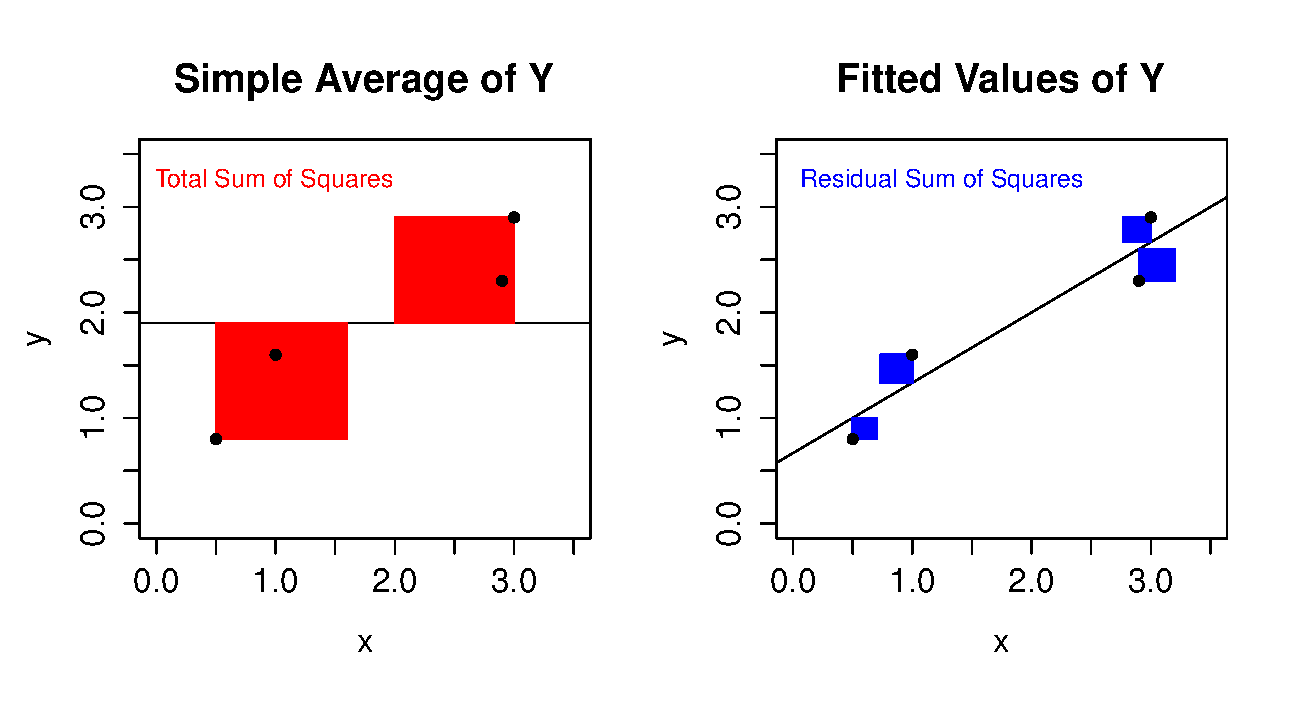
\includegraphics[width=35pc]{regression04}
\caption{$R^2$ is defined generally as $1-\frac{SS_{residual}}{SS_{total}}$. Here, we see the total sum of squares (red) as the sum of the squared distance from each observation to the arithmetic mean of $y$ ($\bar{y}$). The residual sum of squares (blue) is computed as the sum of the squared distance from each observation to its predicted value.}
\label{fig:regression04}
\end{figure}

Next we can look at the residual sum of squares, shown in blue on the right. Here we have our line of best fit along with the same four data points. To calculate this sum of squares, we follow the same procedure as before: we measure the distance on the $y$-axis between each data point and the line, we square it, and then we add together all those values. In this case, though, the difference represents the failure of our model to explain the relationship between our two variables. If it explained the relationship perfectly, then our residual sum of squares would be equal to 0.

So, knowing that a larger value of our $SS_{total}$ indicates a stronger relationship and that a smaller value of our $SS_{residual}$ means a better model, we can see that larger values of $R^2$ mean that a larger proportion of the variance seen in our data is explained by the model. (Remember, dividing a small number---$SS_{residual}$---by a larger number---$SS_{total}$---gives you an even smaller result. So if $R^2$ is equal to 1 minus whatever that value is, its value will approach 1 as the model becomes better and 0 as the model becomes worse.

\subsubsection{Residuals in the Context of a Linear Model}

When we construct a regression model, looking at a plot of the fitted values by the residuals can be a good diagnostic tool. (In R we achieve this by calling \verb|plot(resid(fit), fitted(fit)| where \verb|fit| is the linear model that we have created. See our Implementation in R section for details of how to create a linear model.) Figure \ref{fig:regression08} illustrates some common patterns among residual plots.

\begin{figure}[htp]
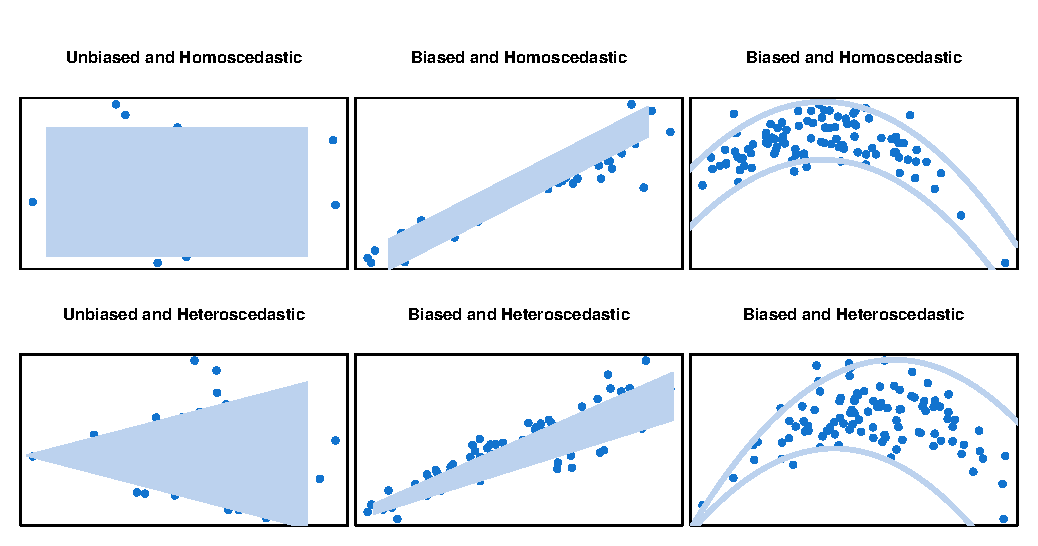
\includegraphics[width=35pc]{regression08}
\caption{Typical patterns for biased and unbiased, heteroscedastic and homoscedastic residuals. Heteroscedasticity means that not all observations in a sample or population have the same variance and usually indicates that the data should be transformed. A residual plot is biased if the fitted values at any given value of the residual do not average out to be 0.}
\label{fig:regression08}
\end{figure}

Here, what we really want to see is something like the graph in the top left---unbiased and homoscedasatic. When this is the case, our residuals will form roughly a rectangle on our plot. It indicates that the model fits our data fairly well. When we start seeing any of the other patterns illustrated, however, that may indicate either that the data need to be transformed or that a different model should be fit differently (e.g., a different type of regression is appropriate).

Unfortunately, the examples given here are all highly stylized: in practice, it's often a much murkier picture that you're left to interpret and make a best guess on. There are some tools to help you that we outline in our chapter on Data Transformations, but by and large this is something that you just need to get a feel for through practice and repeated exposure. Typically, however, bias among your residuals indicates that the model that you chose is not appropriate for your data. Alternately, heteroscedastic residuals usually indicate the need for a data transformation.

\section{Cautions and Considerations}

\subsection{Basic Assumptions}

When running a regression, there are certain conditions that the model assumes are met. These include:
\begin{enumerate}
	\item The data represent a normally-distributed sample of 
	\item 
	\item 
	\item 
\end{enumerate}

\subsection{Outliers and Influential Points}

\section{Implementation in R}

\section{Case Study: Evidence for the Big Bang}

Let's, for throwback Thursday's sake, head back to the late 1920s when physicists were hotly debating models of the universe, whether it was expanding, whether it was an \href{http://en.wikipedia.org/wiki/Steady_state_theory}{eternal steady state universe}, and so forth. Let's say for a moment we're working with Edwin Hubble and we're trying to demonstrate conclusively that in fact the Big Bang is the best cosmological model for the development of the early universe.

But this is a crazy idea! It's heretical! How can we hope to demonstrate its validity? Well, simplifying the story a bit, Hubble realized if this model were true, we could predict the distance of an extra-galactic nebula from Earth using its measured recession velocity. But, you ask, why does this matter? Well, let's take a look at Figure \ref{fig:regression06}

\begin{figure}[htp]

\caption{Movement of galaxies from a central point and all that fun stuff!}
\label{fig:regression06}
\end{figure}

The idea is that, if the Big Bang were the correct model, then it would make sense for us to see galaxies further away from the earth to be receding at a faster speed than those closer to us. If a galaxy were moving in approximately the same direction as ours, then either (1) it would be moving faster than ours; (2) ours would be moving faster than it; or (3) they would be moving at approximately the same speeds. In either case 1 or 2, this would result in the two galaxies moving further apart. In the third case, as long as the two are not moving in exactly the same direction (i.e., $\theta \neq 0$ where $\theta$ is the interior angle between the trajectories of the two galaxies), we will also continue to move farther apart (but at a slower rate). And of course if the galaxies are moving in opposite directions, their recession velocity will be greater still.

\begin{figure}[htp]
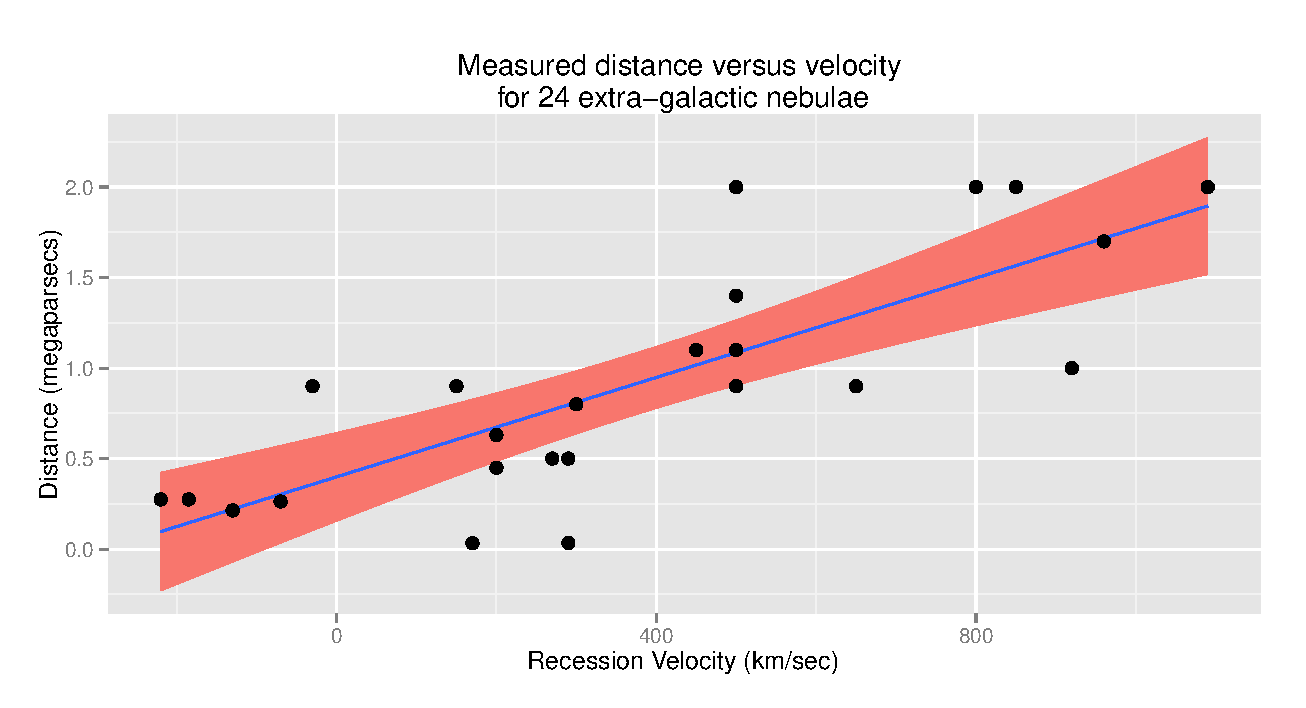
\includegraphics[width=35pc]{regression02}
\caption{Measured distance versus velocity for 24 extra-galactic nebulae. Data from Hubble, E. (1929). \href{http://www.ncbi.nlm.nih.gov/pmc/articles/PMC522427/}{A relation between distance and radial velocity among extra-galactic nebulae.} \textit{Proceedings of the National Academy of Sciences of the United States of America, 15}, 168-173. Line of best fit plotted in blue with a 95\% confidence interval for the regression line in red.}
\label{fig:regression02}
\end{figure}

So, knowing this, we can plot the relationship between recession velocity and distance for the 24 extra-galactic nebulae that Hubble observed (seen in Figure \ref{fig:regression02}). Doing so, we see that there appears to be a positive relationship between the two. Indeed, if we construct a simple linear model, we see:

\begin{framed}
\begin{Verbatim}[samepage=TRUE]
Coefficients:
             Estimate Std. Error t value Pr(>|t|)    
(Intercept) 0.3990982  0.1184697   3.369  0.00277 ** 
Velocity    0.0013729  0.0002274   6.036 4.48e-06 ***

Residual standard error: 0.405 on 22 degrees of freedom
Multiple R-squared:  0.6235,	Adjusted R-squared:  0.6064 
F-statistic: 36.44 on 1 and 22 DF,  p-value: 4.477e-06
\end{Verbatim}
\end{framed}

We can see that we have obtained a significant overall model, $F(1,22) = 36.44$; $p\text{-value}<0.001$, with velocity contributing significantly to that model, $t=6.04$; $p\text{-value}<0.001$. This in turn gives us the ability to predict a galaxy's distance from Earth given its recession velocity, via the formula:
\begin{equation*}
\text{Distance}=0.399+0.00137\cdot\text{Velocity}
\end{equation*}

Moreover, looking at a plot of our fitted valued by our residuals (Figure \ref{fig:regression07}), we see that it appears approximately unbiased and homoscedastic, indicating that we likely have a well-fitted model and that our data don't need to be transformed in any way. Given all this, we can fairly conclude that there is a relationship between the distance of an extra-galactic nebula from Earth and its recession velocity, implying that, indeed, all bodies in the universe are moving apart from one another, having originated from a central point at one time in the universe's history. That is, we find significant support for the Big Bang Theory.

\begin{figure}[htp]
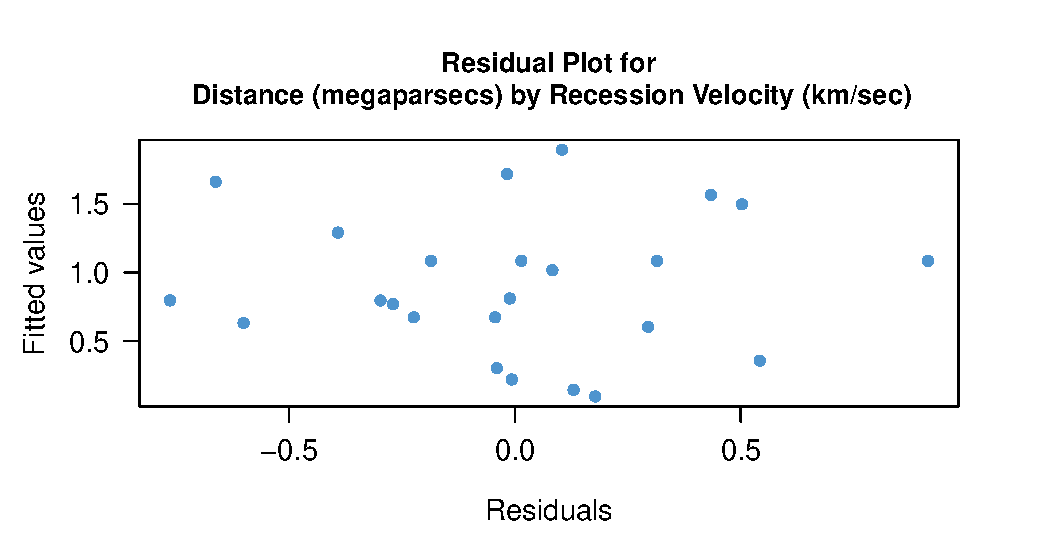
\includegraphics[width=35pc]{regression07}
\caption{Regression plot for our linear model predicting extra-galactic nebula distance by recession velocity}
\label{fig:regression07}
\end{figure}
\section{Exercises}

\section{Additional resources}